\linebreak
In this chapter I aim to describe the proposed architecture of the solution, starting with a high-level glance -- the component diagram.

The smart wearable gadget will require an application to propagate the data from the heart rate sensor to the smart phone application.
Once the raw data is received, it is combined with GPS data and forwarded through the 'biometric and GPS raw data exchange' interface to the IoT platform, where it gets processed and saved.
When the smart phone application requires it, it requests the processed data through the 'processed data retrieval' and displays it.

\begin{figure}[h]
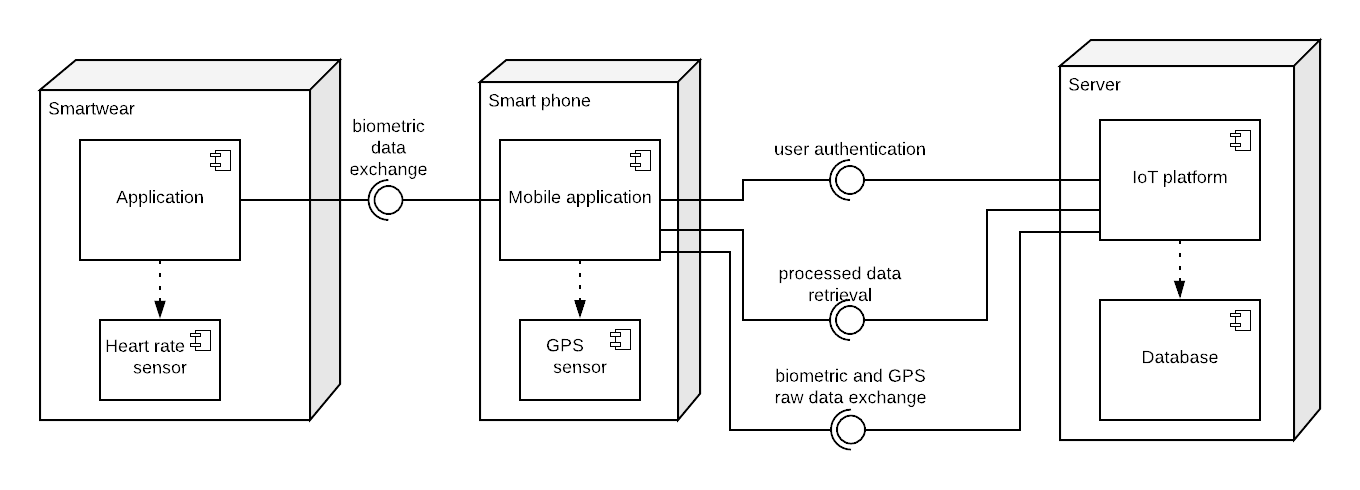
\includegraphics[width=\textwidth]{component.png}
\end{figure}